\documentclass[tikz,border=8pt]{standalone}
% Shared look for every TikZ diagram. Load with \input{../../tools/tikz-style.tex}
\usepackage[sfdefault]{roboto}
\usetikzlibrary{arrows.meta, positioning, shapes.geometric, calc, fit, backgrounds}
\definecolor{cblue}{HTML}{4C78A8}
\definecolor{corange}{HTML}{F58518}
\definecolor{cgreen}{HTML}{54A24B}
\definecolor{cred}{HTML}{E45756}
\definecolor{cpurple}{HTML}{B279A2}
\definecolor{cgrey}{HTML}{6B6B6B}
\tikzset{
  every picture/.style={font=\sffamily, line width=1.2pt},
  box/.style={draw=#1, fill=#1!12, rounded corners=4pt, align=center, inner sep=7pt, minimum height=1.1cm},
  box/.default=cgrey,
  arrow/.style={-{Stealth[length=3mm]}, draw=cgrey, line width=1.4pt},
  title/.style={font=\sffamily\bfseries\Large},
  note/.style={font=\sffamily\small, text=cgrey, align=center},
}
\AtBeginDocument{\hyphenpenalty=10000 \exhyphenpenalty=10000}

% Two ways to combine the search over actions with the search over numbers (Garrett et al. 2021, Fig. 11).
% Top: sequence before satisfy, the planner run in this Note. Bottom: satisfy before sequence, PDDLStream's
% incremental algorithm: sample values with the streams, search for a plan that uses only tested values, repeat.
\begin{document}
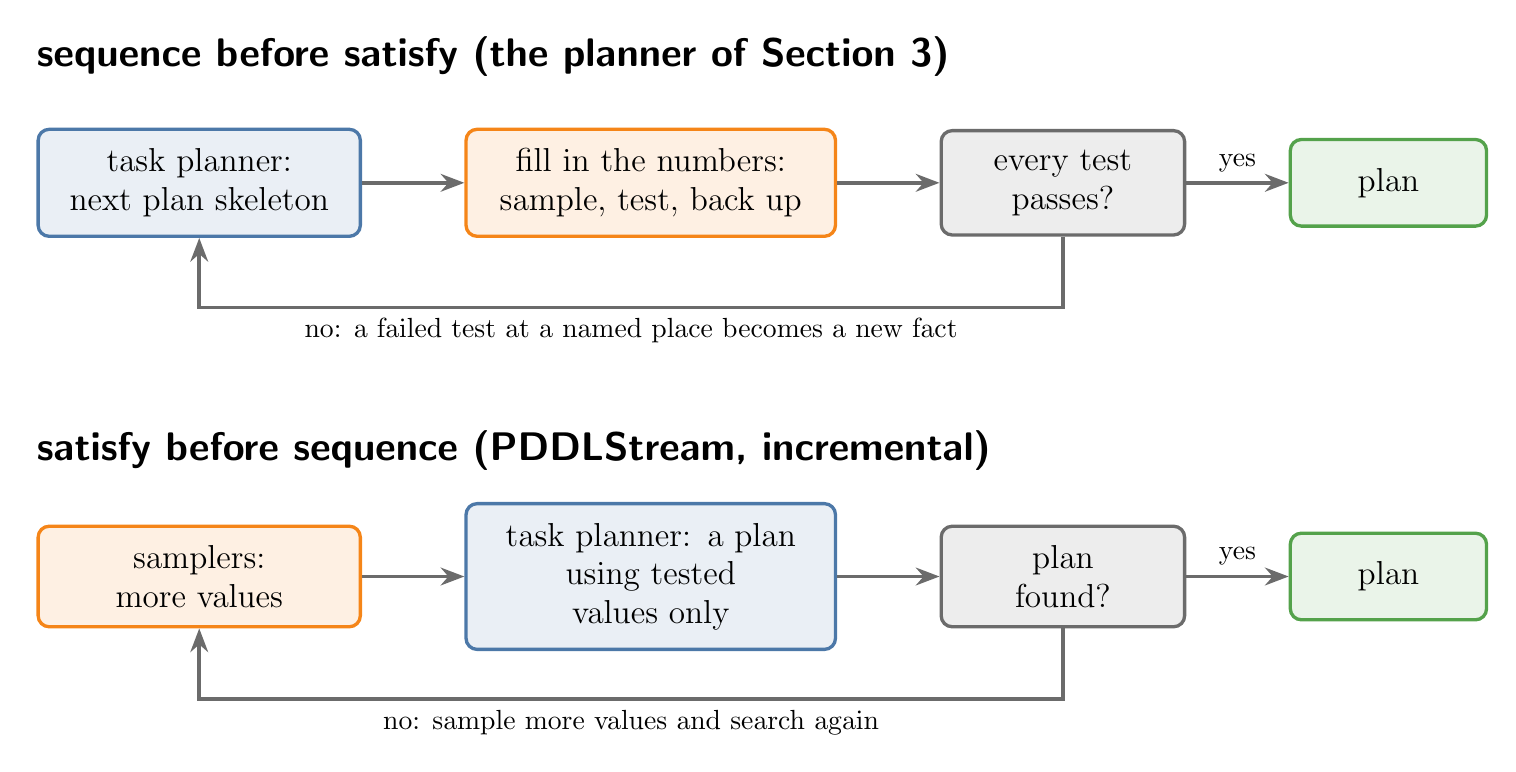
\begin{tikzpicture}[every node/.append style={font=\large}]
  \node[title, anchor=west] at (0, 1.6) {sequence before satisfy (the planner of Section 3)};
  \node[box=cblue, text width=3.6cm] (a1) at (2.2, 0) {task planner:\\ next plan skeleton};
  \node[box=corange, text width=4.2cm, right=1.3cm of a1] (a2) {fill in the numbers:\\ sample, test, back up};
  \node[box=cgrey, text width=2.6cm, right=1.3cm of a2] (a3) {every test\\ passes?};
  \node[box=cgreen, text width=2.0cm, right=1.3cm of a3] (a4) {plan};
  \draw[arrow] (a1) -- (a2);
  \draw[arrow] (a2) -- (a3);
  \draw[arrow] (a3) -- node[above, font=\normalsize] {yes} (a4);
  \draw[arrow] (a3.south) -- ++(0, -0.9) -| node[pos=0.25, below, font=\normalsize]
    {no: a failed test at a named place becomes a new fact} (a1.south);

  \node[title, anchor=west] at (0, -3.4) {satisfy before sequence (PDDLStream, incremental)};
  \node[box=corange, text width=3.6cm] (b1) at (2.2, -5) {samplers:\\ more values};
  \node[box=cblue, text width=4.2cm, right=1.3cm of b1] (b2) {task planner: a plan\\ using tested values only};
  \node[box=cgrey, text width=2.6cm, right=1.3cm of b2] (b3) {plan\\ found?};
  \node[box=cgreen, text width=2.0cm, right=1.3cm of b3] (b4) {plan};
  \draw[arrow] (b1) -- (b2);
  \draw[arrow] (b2) -- (b3);
  \draw[arrow] (b3) -- node[above, font=\normalsize] {yes} (b4);
  \draw[arrow] (b3.south) -- ++(0, -0.9) -| node[pos=0.25, below, font=\normalsize]
    {no: sample more values and search again} (b1.south);
\end{tikzpicture}
\end{document}
